\chapter{Casos de Estudio}

\section{Ejemplo de demostraci'on con file system}

TODO: aplicar las acciones del tutorial.
http://www.dc.uba.ar/inv/grupos/rfm_folder/dynamite/tutorial


\section{B'usqueda de contraejemplo}

A continuaci'on se ejemplifica el an'alisis de una conjectura definida en el lenguaje \textit{Alloy}:

\begin{verbatim}
assert ConjeturaFalsa {
    all o: Dir | some (contents.o)
}
\end{verbatim}

La especificaci'on que se usa para este ejemplo es \textit{file$\_$system.als} \ref{anexo_fs}

Lo primero que se hace es cargar el archivo de especificaci'on que contiene dicha conjecura (\textbf{File$\rightarrow$New Analysis$\rightarrow$Alloy}). Una vez hecha la carga, lo que se quiere demostrar aparece en el nodo raiz:

\begin{figure}[H]
	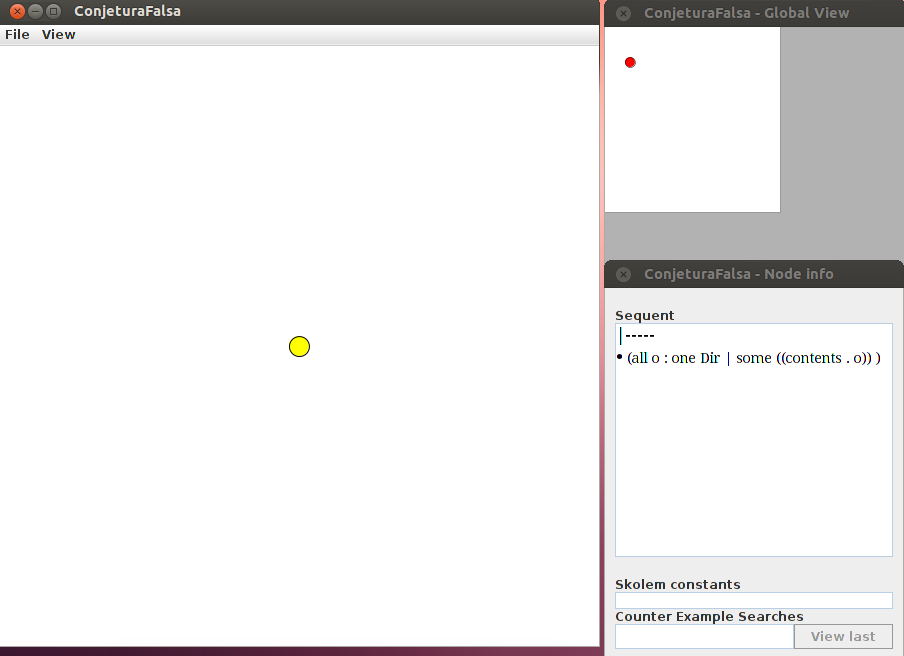
\includegraphics[width=350px]{img/conjetura_falsa_1.png}
	\centering
	\caption{El nodo representa al secuente en el lenguaje \textit{Alloy}}
\end{figure}

A continuaci'on, como se quiere hacer el an'alisis con herramientas de \textit{TPTP-FOF}, es necesario traducir el secuente analizado a \textit{PDOCFA} y luego a \textit{TPTP-FOF}. Las traducciones se realizan seleccionando la opci'on \textbf{$\rho$-translate to PDOCFA} del menu que aparece al hacer click derecho sobre el nodo raiz; y luego aplicando \textbf{$\rho$-translate to TPTP-FOF} haciendo click derecho sobre el nodo resultante de la operaci'on anterior. 

'Esto crea dos nodos nuevos en el 'arbol, representando cada acci'on realizada y mostrando el secuente resultante de las acciones aplicadas:

\begin{figure}[H]
	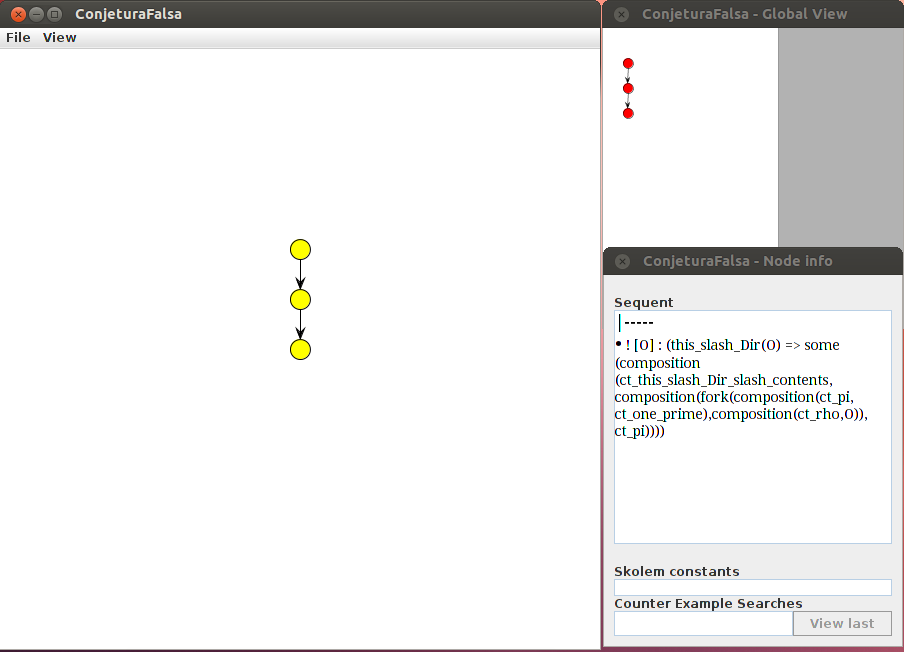
\includegraphics[width=350px]{img/conjetura_falsa_2.png}
	\centering
	\caption{El nodo hoja seleccionado, representa la conjetura inicial traducida al lenguaje \textit{TPTP-FOF}}
\end{figure}

Intuitivamente sospechamos que la conjetura debe ser falsa, ya que est'a diciendo que ``todos los directorios tienen alg'un contenido''. Teniendo 'esto en cuenta, primero probamos realizar una b'usqueda de un contraejemplo con \textit{EProver}, haciendo click derecho sobre el nodo hoja y seleccionando \textbf{Counter Example$\rightarrow$Find Counter Example using EProver for TPTP-FOF}.

Luego de unos segundos el sistema indica que no se pudo encontrar un contraejemplo. 'Este mensaje no indica que el contraejemplo no existe y solamente nos dice que la herramienta no lo encontr'o. Con lo cu'al se puede seguir buscando con otra herramienta.

C'omo ya se realiz'o una acci'on sobre el nodo hoja y no queremos perder la informaci'on del resultado de 'esta acci'on, lo que se hace es crear una rama alternativa para seguir con la demostraci'on manteniendo los resultados en una rama aparte. Al hacer click derecho sobre el nodo y seleccionando \textbf{Modify Tree$\rightarrow$Create an alternative branch} se abren dos ramas salientes del nodo seleccionado. Cada rama est'a representada por una copia del nodo y puede ser analizada en forma independiente del resto.

\begin{figure}[H]
	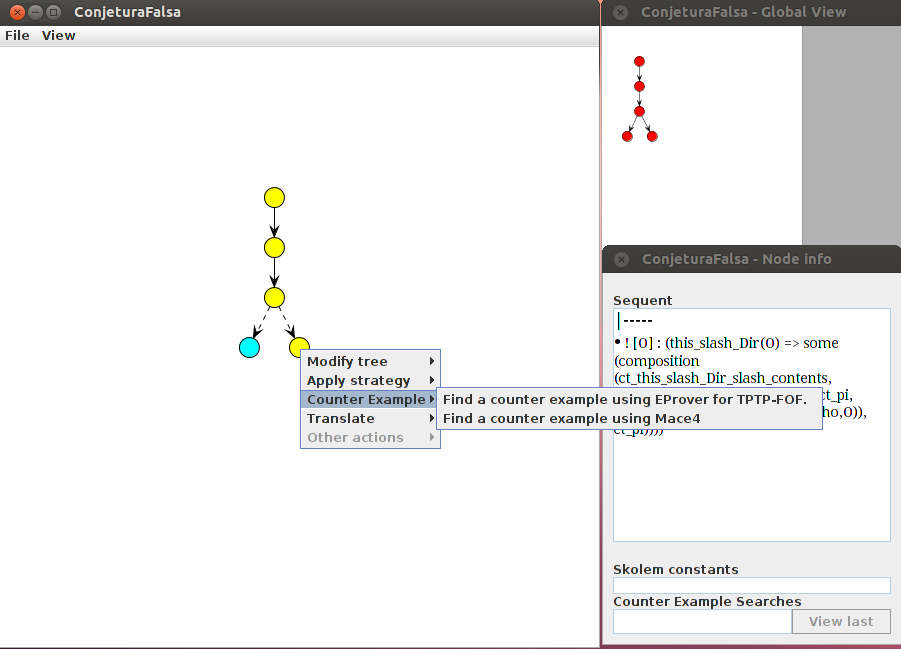
\includegraphics[width=350px]{img/conjetura_falsa_3.png}
	\centering
	\caption{Nodo celeste indica que no se encontr'o un contraejemplo.}
\end{figure}

'Esta ramificaci'on representada con una l'inea punteada se interpreta como un camino alternativo. Alcanza con llegar a un resultado en una de las ramas para afirmar que el resultado vale para el nodo raiz de la ramificaci'on.

Para seguir buscando se intenta una b'usqueda de contraejemplo con otra herramienta, \textit{Mace4}. Al hacer click sobre el nodo de la rama derecha y seleccionando \textbf{Counter Example$\rightarrow$Find a counter example using Mace4} se lanza la operaci'on.

'Esta vez se logra encontrar un contraejemplo y el nodo analizado se pinta de rojo, indicando el resultado exitoso de la operaci'on.

\begin{figure}[H]
	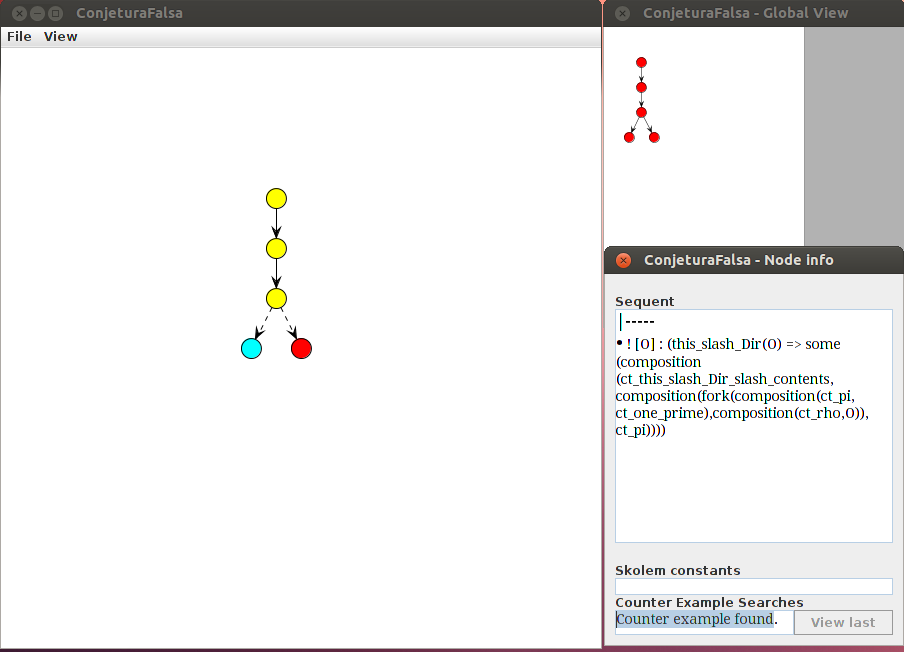
\includegraphics[width=350px]{img/conjetura_falsa_4.png}
	\centering
	\caption{El nodo rojo indica que se encontr'o un contraejemplo}
\end{figure}

Al encontrar un contraejemplo en una ramificaci'on alternativa, se puede afirmar que existe un contraejemplo para el nodo raiz de la ramificaci'on. Luego el contraejemplo es para el secuente en el lenguaje \textit{TPTP-FOF}, pero como es un lenguaje menos expresivo que \textit{PDOCFA} entonces tambi'en existe un contraejemplo para el secuente en \textit{PDOCFA}. Adem'as como la traducci'on entre \textit{Alloy} y \textit{PDOCFA} es sin p'erdida de precisi'on, existe un contraejemplo para el secuente original en \textit{Alloy}. Con lo cu'al se concluye que la conjetura es falsa.


\section{Analisis de lemas XXX}
\label{analisis_lemas}
Como parte del an'alisis y evaluaci'on de los demostradores de teoremas integrados (\textit{EProver} y \textit{SPASS}) evaluamos un conjunto de lemas correspondientes a XXX \ref{anexo_lemas_fof}.

Los lemas se definieron como f'ormulas \textit{PDOCFA}, se aplic'o una traducci'on-$\rho$ a \textit{TPTP-FOF} y se trat'o de demostrar cada lema por separado. C'omo la traducci'on entre \textit{PDOCFA} y \textit{TPTP-FOF} no es exacta, fue necesario especificar un par'ametro numerico $n$ que indica la cantidad de desarrollos que se hacen de la clausura reflexotransitiva.

Para 'estos ejemplo probamos con el par'ametro $n$=$5$, $10$, $20$ y $50$. En todos los casos obtuvimos los mismos resultados:

\vspace{1em}

\begin{tabular}{| l | l | l |}
\hline
  Nombre del lema & Se demostr'o con EProver & Se demostr'o con SPASS  \\\hline
  
M10 & No & No \\
M11b & No & No \\
M12b & Si & Si \\
M13 & No & No \\
M15 & No & No \\
M16 & Si & Si \\
M17 & No & No \\
M18 & No & No \\
M19 & No & No \\
M1h0 & No & No \\
M1M1b & No & No \\
M1M1 & No & No \\
M1M4 & No & No \\
M1M5 & No & No \\
M1M6 & No & No \\
M1M7 & No & No \\
M1 & No & No \\
M20 & No & No \\
M21 & No & No \\
M22 & No & No \\
M23b & No & No \\
M23 & Si & Si \\
M24 & No & No \\
M25 & Si & Si \\
M2 & No & No \\
M30 & No & No \\
M31 & No & No \\
M32 & No & No \\
M4 & No & No \\
M5M1 & No & No \\
M5 & No & No \\
M6M1r2b & Si & Si \\
M6M1r2c & Si & Si \\
M6M1r2 & Si & Si \\
M7 & No & No \\
M8 & No & No \\
M9 & Si & Si \\
Mb2 & No & No \\

\hline
\end{tabular}

\vspace{1em}

Tanto \textit{EProver} como \textit{SPASS} tuvieron el mismo comportamiento y lograron demostrar los mismos lemas.

Analizando cada lema se puede ver que los lemas que fueron demostrados no contienen la operaci'on \textbf{composition}. A su vez los lemas que no tuvieron un resultado positivo, todos conten'ian dicha operaci'on. 

Creemos que el problema reside ah'i, ya que los demostradores tanto \textit{EProver} como  \textit{SPASS} son generales para l'ogica de primer 'orden y es necesario usar t'ecnicas de demostraci'on especificas de 'algebras relacionales al trabajar con las composiciones. En caso contrario, el demostrador puede entrar en un ciclo infinito buscando como realizar la composici'on.


%á